\section{Results}

\begin{figure*}

  \begin{panel}{(a)}{\textwidth}
    \def\histogramcsv{figures/data/sim_counting/intensity_histogram.csv}
    \def\tracecsv{figures/data/sim_counting/trace_and_fit_N10.csv}
    \def\traceintensitycol{trace}
    \def\zcol{fit}
    \def\histbincol{N10_bins}
    \def\histcountcol{N10_measured}
    \def\modelfitcol{N10_model}
    \def\posteriorcsv{figures/data/sim_counting/posteriors.csv}
    \def\posteriorcol{posterior_10}
    \hspace{-2mm}
    \tikzsetnextfilename{figure_2_trace_N10}
    \begin{tikzpicture}
      \node (fancyplot) {\begin{tikzpicture}%
  \begin{axis}[
    name=trace,
    width=0.8\textwidth,
    height=5cm,
    xlabel=frames,
    ylabel=intensity,
    enlarge x limits=false,
    xtick distance=500,
    grid=major,
    grid style={dashed},
    scaled ticks=false,
    ticklabel style={font=\small},
    legend style={nodes={scale=0.6, transform shape}},
  ]

    \addplot [
      color=tracecolor,
      mark=*,
      mark size=0.7pt,
      mark options={line width=0},
      fill opacity=0.8,
      draw opacity=0.2,
    ] table [
      col sep=comma,
      x=frames,
      y=\traceintensitycol
    ] {\tracecsv};
    \addlegendentry{intensity trace}

    \addplot [
      color=ztracecolor,
      thick
    ] table [
      col sep=comma,
      x=frames,
      y=\zcol
    ] {\tracecsv};
    \addlegendentry{inferred state}

    % remember min/max y-axis values for next plot
    \pgfplotsextra{
      \pgfmathparse{\pgfkeysvalueof{/pgfplots/ymin}}
      \global\let\ymin\pgfmathresult
      \pgfmathparse{\pgfkeysvalueof{/pgfplots/ymax}}
      \global\let\ymax\pgfmathresult
    }

  \end{axis}

  \begin{axis}[
    at={($(trace.east) + (4mm,0)$)},
    anchor=west,
    width=0.3\textwidth,
    height=5cm,
    yticklabel=\empty,
    xtick distance=0.005,
    xlabel=probability,
    grid=major,
    grid style={dashed, very thin},
    enlarge x limits={value=0.1,upper},
    scaled ticks=false,
    ymin=\ymin,
    ymax=\ymax,
    ticklabel style={font=\small},
    legend style={nodes={scale=0.6, transform shape}},
  ]

    \addplot+[
      xbar interval,
      mark=none,
      color=tracecolor,
      fill=tracecolor,
      fill opacity=0.6,
      draw=none,
    ] table [
      col sep=comma,
      y=\histbincol,
      x=\histcountcol,
    ] {\histogramcsv};
    \addlegendentry{intensity histogram}

    \addplot[
      color=intensitymodelcolor!80!black,
      thick
    ] table [
      col sep=comma,
      y=\histbincol,
      x=\modelfitcol
    ] {\histogramcsv};
    \addlegendentry{inferred model}

  \end{axis}
\end{tikzpicture}%
};
      \def\noylabels{}
      \def\noxlabel{}
      \node[anchor=south east,text width=12mm]
        at ($(fancyplot.south east)+(-0.6,0.8)$)
        {\@ifundefined{noylabels}{}{%
  \pgfplotsset{yticklabel=\empty}%
}%
\begin{tikzpicture}%

  \def\eps{0.001}

  \begin{axis}[
    width=\textwidth,
    height=\textwidth,
    xlabel=\n,
    xlabel=$p(\n|\trace)$,
    grid=major,
    grid style={dashed, very thin},
    enlarge x limits=0.1,
    enlarge y limits=0,
    ymin=0,
    ymax=1,
    scaled ticks=false,
    ticklabel style={font=\small},
  ]

    \addplot+[
      ybar,
      bar width=1,
      mark=none,
      fill=posteriorcolor,
      fill opacity=0.6,
      draw=posteriorcolor,
      y filter/.expression={
        y < \eps ? nan : y
      },
    ] table [
      col sep=comma,
      y=\posteriorcol,
      x=n,
    ] {\posteriorcsv};

    \ifdefined\posteriorcolextra
      \addplot+[
        ybar,
        bar width=1,
        mark=none,
        fill=posteriorcolor!60!black,
        fill opacity=0.6,
        draw=posteriorcolor,
        y filter/.expression={
          y < \eps ? nan : y
        },
      ] table [
        col sep=comma,
        y=\posteriorcolextra,
        x=n,
      ] {\posteriorcsv};
    \fi

  \end{axis}

\end{tikzpicture}
};
    \end{tikzpicture}

    \vspace{-4mm}
  \end{panel}

  \begin{panel}{(b)}{\textwidth}
    \def\histogramcsv{figures/data/sim_counting/intensity_histogram.csv}
    \def\tracecsv{figures/data/sim_counting/trace_and_fit_N20.csv}
    \def\traceintensitycol{trace}
    \def\zcol{fit}
    \def\histbincol{N20_bins}
    \def\histcountcol{N20_measured}
    \def\modelfitcol{N20_model}
    \def\posteriorcsv{figures/data/sim_counting/posteriors.csv}
    \def\posteriorcol{posterior_20}
    \hspace{-2mm}%
    \tikzsetnextfilename{figure_2_trace_N20}
    \begin{tikzpicture}
      \node (fancyplot) {\begin{tikzpicture}%
  \begin{axis}[
    name=trace,
    width=0.8\textwidth,
    height=5cm,
    xlabel=frames,
    ylabel=intensity,
    enlarge x limits=false,
    xtick distance=500,
    grid=major,
    grid style={dashed},
    scaled ticks=false,
    ticklabel style={font=\small},
    legend style={nodes={scale=0.6, transform shape}},
  ]

    \addplot [
      color=tracecolor,
      mark=*,
      mark size=0.7pt,
      mark options={line width=0},
      fill opacity=0.8,
      draw opacity=0.2,
    ] table [
      col sep=comma,
      x=frames,
      y=\traceintensitycol
    ] {\tracecsv};
    \addlegendentry{intensity trace}

    \addplot [
      color=ztracecolor,
      thick
    ] table [
      col sep=comma,
      x=frames,
      y=\zcol
    ] {\tracecsv};
    \addlegendentry{inferred state}

    % remember min/max y-axis values for next plot
    \pgfplotsextra{
      \pgfmathparse{\pgfkeysvalueof{/pgfplots/ymin}}
      \global\let\ymin\pgfmathresult
      \pgfmathparse{\pgfkeysvalueof{/pgfplots/ymax}}
      \global\let\ymax\pgfmathresult
    }

  \end{axis}

  \begin{axis}[
    at={($(trace.east) + (4mm,0)$)},
    anchor=west,
    width=0.3\textwidth,
    height=5cm,
    yticklabel=\empty,
    xtick distance=0.005,
    xlabel=probability,
    grid=major,
    grid style={dashed, very thin},
    enlarge x limits={value=0.1,upper},
    scaled ticks=false,
    ymin=\ymin,
    ymax=\ymax,
    ticklabel style={font=\small},
    legend style={nodes={scale=0.6, transform shape}},
  ]

    \addplot+[
      xbar interval,
      mark=none,
      color=tracecolor,
      fill=tracecolor,
      fill opacity=0.6,
      draw=none,
    ] table [
      col sep=comma,
      y=\histbincol,
      x=\histcountcol,
    ] {\histogramcsv};
    \addlegendentry{intensity histogram}

    \addplot[
      color=intensitymodelcolor!80!black,
      thick
    ] table [
      col sep=comma,
      y=\histbincol,
      x=\modelfitcol
    ] {\histogramcsv};
    \addlegendentry{inferred model}

  \end{axis}
\end{tikzpicture}%
};
      \def\noylabels{}
      \def\noxlabel{}
      \node[anchor=south east,text width=12mm]
        at ($(fancyplot.south east)+(-0.6,0.8)$)
        {\@ifundefined{noylabels}{}{%
  \pgfplotsset{yticklabel=\empty}%
}%
\begin{tikzpicture}%

  \def\eps{0.001}

  \begin{axis}[
    width=\textwidth,
    height=\textwidth,
    xlabel=\n,
    xlabel=$p(\n|\trace)$,
    grid=major,
    grid style={dashed, very thin},
    enlarge x limits=0.1,
    enlarge y limits=0,
    ymin=0,
    ymax=1,
    scaled ticks=false,
    ticklabel style={font=\small},
  ]

    \addplot+[
      ybar,
      bar width=1,
      mark=none,
      fill=posteriorcolor,
      fill opacity=0.6,
      draw=posteriorcolor,
      y filter/.expression={
        y < \eps ? nan : y
      },
    ] table [
      col sep=comma,
      y=\posteriorcol,
      x=n,
    ] {\posteriorcsv};

    \ifdefined\posteriorcolextra
      \addplot+[
        ybar,
        bar width=1,
        mark=none,
        fill=posteriorcolor!60!black,
        fill opacity=0.6,
        draw=posteriorcolor,
        y filter/.expression={
          y < \eps ? nan : y
        },
      ] table [
        col sep=comma,
        y=\posteriorcolextra,
        x=n,
      ] {\posteriorcsv};
    \fi

  \end{axis}

\end{tikzpicture}
};
    \end{tikzpicture}
  \end{panel}

  \begin{panel}{(c)}{0.45\textwidth}
    \def\posteriormatrixcsv{figures/data/sim_counting/heatmap.csv}
    \def\lbfcscsv{figures/data/sim_counting/heatmap_lbfcs.csv}
    \tikzexternaldisable
    \tikzsetnextfilename{figure_2_lbfcs_comparison}
    \begin{tikzpicture}
  \begin{axis}[
    name=trace,
    width=\textwidth,
    height=\textwidth,
    xlabel=Estimated \n,
    ylabel=True \n,
    enlarge x limits=false,
    enlarge y limits=false,
    grid=major,
    grid style={dashed},
    scaled ticks=false,
    ticklabel style={font=\small},
    xtick align=outside,
    xtick pos=lower,
    ytick align=outside,
    ytick pos=lower,
    colorbar,
  ]

    \pgfplotsset{
      colormap={posteriorcolormap}{
        color(0.0)=(white)
        color(0.2)=(funkey_color_2)
        color(1.0)=(funkey_color_2!50!black)
      }
    }

    \addplot[
      matrix plot*,
      mesh/cols=35,
      point meta=explicit,
    ] table [
      col sep=comma,
      x=n,
      y=true_n,
      meta=posterior,
    ] {\posteriormatrixcsv};

  \end{axis}

  \begin{axis}[
    name=trace,
    width=\textwidth,
    height=\textwidth,
    xmin=0.5,
    xmax=35.5,
    ymin=0.5,
    ymax=30.5,
    grid=major,
    grid style={dashed},
    scaled ticks=false,
    domain=0:35,
    ticklabel style={font=\small},
  ]

    \addplot[
      mark=*,
      only marks,
      mark size=1.4pt,
      mark options={draw=white,fill=funkey_color_1,draw opacity=0.6,fill opacity=0.7},
    ] table [
      col sep=comma,
      x=lbfcs_count,
      y=n,
    ] {\lbfcscsv};

    \addplot[no marks,thick,gray] {x};

  \end{axis}

\end{tikzpicture}

    \tikzexternalenable
  \end{panel}
  \hspace{1cm}
  \begin{panel}{(d)}{0.5\textwidth}
    \begin{panel}{}{\textwidth}
      \vspace{2mm}
      \hspace{2mm}
      \small
      \def\tracelengthcsv{figures/data/trace_length/trace_length_results.csv}
      \def\mapcol{max_likelihoods_20}
      \def\varcol{variance_20}
      \tikzexternaldisable
      \tikzsetnextfilename{figure_2_trace_length}
      \def\intervalplot#1#2{%
  \addplot[%
    color=#2,%
    very thick,%
  ] table [%
    col sep=comma,%
    x=length,%
    y=max_likelihoods_#1,%
  ] {\tracelengthcsv};%
  \addplot[%
    name path=lower,%
    draw=none,%
    fill=none,%
    forget plot,%
  ] table [%
    col sep=comma,%
    x=length,%
    y expr=\thisrow{max_likelihoods_#1} - \thisrow{variance_#1}%
  ] {\tracelengthcsv};%
  \addplot[%
    name path=upper,%
    draw=none,%
    fill=none,%
    forget plot,%
  ] table [%
    col sep=comma,%
    x=length,%
    y expr=\thisrow{max_likelihoods_#1} + \thisrow{variance_#1}%
  ] {\tracelengthcsv};%
  \addplot [%
    color=#2,%
    opacity=0.4,%
    forget plot,%
  ] fill between[of=lower and upper];%
  \addlegendentry{$n=#1$};
}%
\begin{tikzpicture}
  \begin{axis}[
    width=\textwidth,
    height=0.47\textwidth,
    xlabel={length [frames]},
    %ylabel=estimated count,
    enlarge x limits=false,
    enlarge y limits=false,
    xtick distance=4000,
    ytick distance=5,
    ymin=0,
    grid=major,
    grid style={dashed},
    scaled ticks=false,
    ticklabel style={font=\small},
    legend columns=4,
    legend style={nodes={scale=0.6, transform shape}},
  ]
    \intervalplot{20}{funkey_color_1}
    \intervalplot{15}{funkey_color_2}
    \intervalplot{10}{funkey_color_3}
    \intervalplot{5}{funkey_color_4}
  \end{axis}
\end{tikzpicture}%

      \tikzexternalenable
    \end{panel}
    \begin{panel}{(e)}{\textwidth}
      \hspace{2mm}
      \small
      \def\tracelengthcsv{figures/data/trace_length/trace_length_results.csv}
      \def\mapcol{max_likelihoods_20}
      \def\varcol{variance_20}
      \tikzexternaldisable
      \tikzsetnextfilename{figure_2_trace_length}
      \def\intervalplot#1#2{%
  \addplot[%
    color=#2,%
    very thick,%
  ] table [%
    col sep=comma,%
    x=length,%
    y=max_likelihoods_#1,%
  ] {\tracelengthcsv};%
  \addplot[%
    name path=lower,%
    draw=none,%
    fill=none,%
    forget plot,%
  ] table [%
    col sep=comma,%
    x=length,%
    y expr=\thisrow{max_likelihoods_#1} - \thisrow{variance_#1}%
  ] {\tracelengthcsv};%
  \addplot[%
    name path=upper,%
    draw=none,%
    fill=none,%
    forget plot,%
  ] table [%
    col sep=comma,%
    x=length,%
    y expr=\thisrow{max_likelihoods_#1} + \thisrow{variance_#1}%
  ] {\tracelengthcsv};%
  \addplot [%
    color=#2,%
    opacity=0.4,%
    forget plot,%
  ] fill between[of=lower and upper];%
  \addlegendentry{$n=#1$};
}%
\begin{tikzpicture}
  \begin{axis}[
    width=\textwidth,
    height=0.47\textwidth,
    xlabel={length [frames]},
    %ylabel=estimated count,
    enlarge x limits=false,
    enlarge y limits=false,
    xtick distance=4000,
    ytick distance=5,
    ymin=0,
    grid=major,
    grid style={dashed},
    scaled ticks=false,
    ticklabel style={font=\small},
    legend columns=4,
    legend style={nodes={scale=0.6, transform shape}},
  ]
    \intervalplot{20}{funkey_color_1}
    \intervalplot{15}{funkey_color_2}
    \intervalplot{10}{funkey_color_3}
    \intervalplot{5}{funkey_color_4}
  \end{axis}
\end{tikzpicture}%

      \tikzexternalenable
    \end{panel}
  \end{panel}

  \caption{
    \panelref{a, b} Trace simulated from 10/20 emitters, and the posterior
    distribution estimated by \ours.
    %
    \panelref{c} The \ours posterior is able to accurately estimate
    significantly higher molecular counts than the current state of the art,
    lbFCS
    %
    \panelref{d} As trace length increases, the variance of the \ours posterior
    decreases.
    %
    \panelref{e} As the signal to noise ratio increases the variance of the
    \ours posterior decreases.
  }
  \label{fig:method:overview}

\end{figure*}

\begin{figure*}

  \begin{panel}{(a)}{0.58\textwidth}
    \small%
    \setlength\plotwidth{42mm}%
    \setlength\plotheight{60mm}%
    \begin{tikzpicture}
  \begin{axis}[
    width=\plotwidth,
    height=\plotheight,
    scale only axis=true,
    name=sweep,
    xlabel=\pon,
    ylabel=\poff,
    enlarge x limits=false,
    enlarge y limits=false,
    scaled ticks=false,
    ticklabel style={/pgf/number format/.cd,fixed,precision=3},
    xtick distance=0.04,
    xtick align=outside,
    xtick pos=lower,
    ytick align=outside,
    ytick pos=lower,
    colorbar,
  ]

    \pgfplotsset{
      colormap={posteriorcolormap}{
        color(0.0)=(funkey_color_2!50!white)
        color(0.1)=(funkey_color_2)
        color(0.9)=(funkey_color_1)
        color(1.0)=(funkey_color_1!50!black)
      }
    }

    \addplot[
      matrix plot*,
      mesh/cols=10,
      point meta=explicit,
    ] table [
      col sep=comma,
      x=p_on,
      y=p_off,
      meta=error,
    ] {\kineticsheatmapcsv};

    % highlight qpaint and lbfcs points
    \node[circle,draw=funkey_color_9,thick] (qpaint) at (axis cs:0.01, 0.2) {};
    \node[circle,draw=funkey_color_9,thick] (lbfcs) at (axis cs:0.02, 0.02) {};

  \end{axis}

  \node[anchor=north] (qpaint_zs) at ($(sweep.north east)+(2.8,0)$) {
    \def\zhistogramcsv{figures/data/kinetics_grid/state_histogram.csv}%
    \def\zhistogramcol{qpaint}%
    \def\noylabels{}%
    \setlength\plotwidth{14mm}%
    \setlength\plotheight{16mm}%
    \tikz{\@ifundefined{noylabels}{}{%
  \pgfplotsset{yticklabel=\empty}%
}%
\@ifundefined{noxlabel}{%
  \pgfplotsset{xlabel=\z{}}%
}{%
  \pgfplotsset{xlabel=\empty}%
}%
\begin{axis}[
  width=\plotwidth,
  height=\plotheight,
  scale only axis=true,
  grid=major,
  grid style={dashed, very thin},
  enlarge x limits=0.1,
  enlarge y limits={value=0.2,upper},
  ymin=0,
  scaled ticks=false,
]

  \addplot+[
    ybar,
    bar width=1,
    mark=none,
    fill=ztracecolor,
    fill opacity=0.6,
    draw=ztracecolor,
  ] table [
    col sep=comma,
    y=\zhistogramcol,
    x=bin,
  ] {\zhistogramcsv};

\end{axis}
}%
  };
  \node[fit=(qpaint_zs),inner sep=0,rounded corners,draw=funkey_color_9,thick] (qpaint_box) {};

  \node[anchor=south] (lbfcs_zs) at (sweep.south-|qpaint_zs.south) {
    \def\zhistogramcsv{figures/data/kinetics_grid/state_histogram.csv}%
    \def\zhistogramcol{lbfcs}%
    \def\noylabels{}%
    \setlength\plotwidth{14mm}%
    \setlength\plotheight{16mm}%
    \tikz{\@ifundefined{noylabels}{}{%
  \pgfplotsset{yticklabel=\empty}%
}%
\@ifundefined{noxlabel}{%
  \pgfplotsset{xlabel=\z{}}%
}{%
  \pgfplotsset{xlabel=\empty}%
}%
\begin{axis}[
  width=\plotwidth,
  height=\plotheight,
  scale only axis=true,
  grid=major,
  grid style={dashed, very thin},
  enlarge x limits=0.1,
  enlarge y limits={value=0.2,upper},
  ymin=0,
  scaled ticks=false,
]

  \addplot+[
    ybar,
    bar width=1,
    mark=none,
    fill=ztracecolor,
    fill opacity=0.6,
    draw=ztracecolor,
  ] table [
    col sep=comma,
    y=\zhistogramcol,
    x=bin,
  ] {\zhistogramcsv};

\end{axis}
}%
  };
  \node[fit=(lbfcs_zs),inner sep=0,rounded corners,draw=funkey_color_9,thick] (lbfcs_box) {};

  \draw[funkey_color_3,thick] (qpaint) -- (qpaint-|qpaint_box.west);
  \draw[funkey_color_3,thick] (lbfcs) -- (lbfcs-|lbfcs_box.west);

\end{tikzpicture}

  \end{panel}
  \begin{panel}{(b)}{0.42\textwidth}
    \setlength\plotwidth{56mm}%
    \setlength\plotheight{60mm}%
    \pgfplotsset{/pgf/number format/.cd,fixed,precision=3}%
\begin{tikzpicture}
  \begin{axis}[
    width=\plotwidth,
    height=\plotheight,
    scale only axis=true,
    xlabel=\pon,
    ylabel=\poff,
    grid=major,
    grid style={dashed},
    scaled ticks=false,
    ticklabel style={font=\small},
  ]
    \pgfplotsset{
      colormap={posteriorcolormap}{
        color(0.0)=(funkey_color_7)
        color(0.5)=(funkey_color_2)
        color(1.0)=(funkey_color_1!50!red)
      }
    }

    \addplot[
      patch,
      patch type=rectangle,
      shader=interp,
      draw=black,
      fill opacity=0.4,
    ] table[
      x=pon_mean,
      y=poff_mean,
      point meta=\thisrow{temperature},
    ] {
      pon_mean    pon_var       poff_mean   poff_var      temperature concentration
      0.02813685  8.5348165e-06 0.07232066  9.0882335e-05 25          10
      0.02797574  1.8311839e-05 0.04775255  5.822931e-05  18          10
      0.05270538  6.0997234e-05 0.04954245  4.0005598e-05 18          20
      0.059536304 5.9824146e-05 0.08741606  0.00014375064 25          20

      0.05270538  6.0997234e-05 0.04954245  4.0005598e-05 18          20
      0.059536304 5.9824146e-05 0.08741606  0.00014375064 25          20
      0.07053028  4.2747815e-05 0.10869306  8.929498e-05  25          30
      0.072243474 0.00016735448 0.05488883  0.0012168097  18          30

      0.02797574  1.8311839e-05 0.04775255  5.822931e-05  18          10
      0.05270538  6.0997234e-05 0.04954245  4.0005598e-05 18          20
      0.045684416 6.31415e-05   0.03472516  8.919405e-05  13          20
      0.024452658 2.4062621e-05 0.036942866 4.378218e-05  13          10

      0.05270538  6.0997234e-05 0.04954245  4.0005598e-05 18          20
      0.072243474 0.00016735448 0.05488883  0.0012168097  18          30
      0.052961048 0.00010537513 0.03289487  6.0903745e-05 13          30
      0.045684416 6.31415e-05   0.03472516  8.919405e-05  13          20
    };

    \addplot[
      scatter,
      mark=*,
      only marks,
      point meta=\thisrow{temperature},
      scatter/@pre marker code/.append style={
        /tikz/mark size=\size,
      },
      visualization depends on={\thisrow{concentration} \as \concentration},
      visualization depends on={2+\thisrow{concentration}*0.1 \as \size},
    ] table [
      col sep=comma,
      x=pon_mean,
      y=poff_mean,
    ] {\kineticscsv};

    \coordinate (n_25_10) at (axis cs:0.02813685,0.07232066) {};
    \coordinate (n_18_10) at (axis cs:0.02797574,0.04775255) {};
    \coordinate (n_13_10) at (axis cs:0.024452658,0.036942866) {};
    \coordinate (n_25_20) at (axis cs:0.059536304,0.08741606) {};
    \coordinate (n_18_20) at (axis cs:0.05270538,0.04954245) {};
    \coordinate (n_13_20) at (axis cs:0.045684416,0.03472516) {};
    \coordinate (n_25_30) at (axis cs:0.07053028,0.10869306) {};
    \coordinate (n_18_30) at (axis cs:0.072243474,0.05488883) {};
    \coordinate (n_13_30) at (axis cs:0.052961048,0.03289487) {};

    \begin{pgfonlayer}{background}
      \draw (n_13_10) -- node[pos=0.5,above,sloped] {\tiny10nM} (n_18_10) -- (n_25_10);
      \draw (n_13_20) -- node[pos=0.5,above,sloped] {\tiny20nM} (n_18_20) -- (n_25_20);
      \draw (n_13_30) -- node[pos=0.5,above,sloped] {\tiny30nM} (n_18_30) -- (n_25_30);
      \draw (n_13_10) -- node[pos=0.5,above,sloped] {\tiny$T=13$} (n_13_20) -- (n_13_30);
      \draw (n_18_10) -- node[pos=0.5,above,sloped] {\tiny$T=18$} (n_18_20) -- (n_18_30);
      \draw (n_25_10) -- node[pos=0.5,above,sloped] {\tiny$T=25$} (n_25_20) -- (n_25_30);
    \end{pgfonlayer}
  \end{axis}

\end{tikzpicture}%

  \end{panel}

  \begin{panel}{(c)}{\textwidth}
    \small%
    \setlength\plotwidth{\textwidth}%
    \setlength\plotheight{36mm}%
    \def\tracecsv{figures/data/kinetics_grid/traces.csv}%
\def\traceintensitycol{qpaint_trace}%
\def\zcol{qpaint_fit}%
\def\histogramcsv{figures/data/kinetics_grid/intensity_histogram.csv}%
\def\histbincol{qpaint_bins}%
\def\histcountcol{qpaint_measured}%
\def\modelfitcol{qpaint_model}%
\def\posteriorcsv{figures/data/kinetics_grid/posteriors.csv}%
\def\posteriorcol{qpaint}%
\tikzsetnextfilename{sim_trace_qpaint}%
\begin{tikzpicture}
  \def\plotlabel{$\n = 10$}
  \@ifundefined{nolabels}{
  \pgfplotsset{xlabel=frames}
  \pgfplotsset{ylabel=intensity}
  \pgfplotsset{grid=major}
  \pgfplotsset{grid style={dashed}}
}{
  \pgfplotsset{xticklabel=\empty}
  \pgfplotsset{yticklabel=\empty}
  \pgfplotsset{ticks=none}
  \pgfplotsset{scaled ticks=false}
}
\@ifundefined{histogramcsv}{}{
  \setlength{\plotwidth}{0.73\plotwidth}
}
\begin{axis}[
  name=trace,
  width=\plotwidth,
  height=\plotheight,
  scale only axis=true,
  enlarge x limits=false,
  xtick distance=500,
  ticklabel style={font=\small},
  legend style={fill=black, nodes={scale=0.6, transform shape}},
]

  \addplot [
    color=tracecolor,
    mark=*,
    mark size=0.7pt,
    mark options={line width=0},
    fill opacity=0.8,
    draw opacity=0.0,
  ] table [
    col sep=comma,
    x=frames,
    y=\traceintensitycol
  ] {\tracecsv};
  \@ifundefined{nolabels}{\addlegendentry{intensity trace}}{}

  \@ifundefined{zcol}{}{
    \addplot [
      color=ztracecolor,
      thick
    ] table [
      col sep=comma,
      x=frames,
      y=\zcol
    ] {\tracecsv};
    \@ifundefined{nolabels}{\addlegendentry{inferred state}}{}
  }

  % remember min/max y-axis values for next plot
  \pgfplotsextra{
    \pgfmathparse{\pgfkeysvalueof{/pgfplots/ymin}}
    \global\let\ymin\pgfmathresult
    \pgfmathparse{\pgfkeysvalueof{/pgfplots/ymax}}
    \global\let\ymax\pgfmathresult
  }

\end{axis}
\@ifundefined{plotlabel}{}{
  \node[anchor=north west,rectangle,draw,fill=black] at (trace.north west) {\plotlabel};
}

\@ifundefined{histogramcsv}{}{
  \begin{axis}[
    at={($(trace.east) + (4mm,0)$)},
    name=histogram,
    anchor=west,
    width=0.25\plotwidth,
    height=\plotheight,
    scale only axis=true,
    ylabel=\empty,
    yticklabel=\empty,
    xtick distance=0.01,
    xlabel=probability,
    grid=major,
    grid style={dashed, very thin},
    enlarge x limits={value=0.4,upper},
    scaled ticks=false,
    ymin=\ymin,
    ymax=\ymax,
    ticklabel style={font=\small},
    legend style={fill=black, nodes={scale=0.6, transform shape}},
  ]

    \addplot+[
      xbar interval,
      mark=none,
      color=tracecolor,
      fill=tracecolor,
      fill opacity=0.6,
      draw=none,
    ] table [
      col sep=comma,
      y=\histbincol,
      x=\histcountcol,
    ] {\histogramcsv};
    \addlegendentry{intensity histogram}

    \addplot[
      color=intensitymodelcolor!80!black,
      thick
    ] table [
      col sep=comma,
      y=\histbincol,
      x=\modelfitcol
    ] {\histogramcsv};
    \addlegendentry{inferred model}

  \end{axis}
}

  \def\noylabels{}
  \def\noxlabel{}
  \setlength\plotwidth{0.1\plotwidth}
  \setlength\plotheight{\plotwidth}
  \pgfplotsset{every axis/.style={
    anchor=below south east,
    at={($(histogram.south east)-(2mm,-4mm)$)},
    xtick distance=10
  }}
  \def\eps{0.001}%  skip bars for values below eps
\@ifundefined{noylabels}{}{
  \pgfplotsset{yticklabel=\empty}
  \pgfplotsset{ylabel=\empty}
}
\@ifundefined{noxlabel}{
  \pgfplotsset{xlabel=$n$}
}{
  \pgfplotsset{xlabel=\empty}
}
\begin{axis}[
  width=\plotwidth,
  height=\plotheight,
  scale only axis=true,
  enlarge x limits={abs=1.5},
  enlarge y limits=0,
  ymin=0,
  ymax=1,
  scaled ticks=false,
  ticklabel style={font=\tiny},
  xtick distance=1,
  axis background/.style={fill=white},
]

  \addplot+[
    ybar,
    bar width=1,
    mark=none,
    fill=posteriorcolor,
    fill opacity=0.6,
    draw=posteriorcolor,
    y filter/.expression={
      y < \eps ? nan : y
    },
  ] table [
    col sep=comma,
    y=\posteriorcol,
    x=n,
  ] {\posteriorcsv};

  \ifdefined\posteriorcolextra
    \addplot+[
      ybar,
      bar width=1,
      mark=none,
      fill=posteriorcolor!60!black,
      fill opacity=0.6,
      draw=posteriorcolor,
      y filter/.expression={
        y < \eps ? nan : y
      },
    ] table [
      col sep=comma,
      y=\posteriorcolextra,
      x=n,
    ] {\posteriorcsv};
  \fi

\end{axis}

\end{tikzpicture}
%
    \vspace{-4mm}%
  \end{panel}

  \begin{panel}{(d)}{\textwidth}
    \small%
    \setlength\plotwidth{\textwidth}%
    \setlength\plotheight{36mm}%
    \def\tracecsv{figures/data/kinetics_grid/traces.csv}%
\def\traceintensitycol{lbfcs_trace}%
\def\zcol{lbfcs_fit}%
\def\histogramcsv{figures/data/kinetics_grid/intensity_histogram.csv}%
\def\histbincol{lbfcs_bins}%
\def\histcountcol{lbfcs_measured}%
\def\modelfitcol{lbfcs_model}%
\def\posteriorcsv{figures/data/kinetics_grid/posteriors.csv}%
\def\posteriorcol{lbfcs}%
\tikzsetnextfilename{sim_trace_lbfcs}%
\begin{tikzpicture}
  \def\plotlabel{$\n = 10$}
  \@ifundefined{nolabels}{
  \pgfplotsset{xlabel=frames}
  \pgfplotsset{ylabel=intensity}
  \pgfplotsset{grid=major}
  \pgfplotsset{grid style={dashed}}
}{
  \pgfplotsset{xticklabel=\empty}
  \pgfplotsset{yticklabel=\empty}
  \pgfplotsset{ticks=none}
  \pgfplotsset{scaled ticks=false}
}
\@ifundefined{histogramcsv}{}{
  \setlength{\plotwidth}{0.73\plotwidth}
}
\begin{axis}[
  name=trace,
  width=\plotwidth,
  height=\plotheight,
  scale only axis=true,
  enlarge x limits=false,
  xtick distance=500,
  ticklabel style={font=\small},
  legend style={fill=black, nodes={scale=0.6, transform shape}},
]

  \addplot [
    color=tracecolor,
    mark=*,
    mark size=0.7pt,
    mark options={line width=0},
    fill opacity=0.8,
    draw opacity=0.0,
  ] table [
    col sep=comma,
    x=frames,
    y=\traceintensitycol
  ] {\tracecsv};
  \@ifundefined{nolabels}{\addlegendentry{intensity trace}}{}

  \@ifundefined{zcol}{}{
    \addplot [
      color=ztracecolor,
      thick
    ] table [
      col sep=comma,
      x=frames,
      y=\zcol
    ] {\tracecsv};
    \@ifundefined{nolabels}{\addlegendentry{inferred state}}{}
  }

  % remember min/max y-axis values for next plot
  \pgfplotsextra{
    \pgfmathparse{\pgfkeysvalueof{/pgfplots/ymin}}
    \global\let\ymin\pgfmathresult
    \pgfmathparse{\pgfkeysvalueof{/pgfplots/ymax}}
    \global\let\ymax\pgfmathresult
  }

\end{axis}
\@ifundefined{plotlabel}{}{
  \node[anchor=north west,rectangle,draw,fill=black] at (trace.north west) {\plotlabel};
}

\@ifundefined{histogramcsv}{}{
  \begin{axis}[
    at={($(trace.east) + (4mm,0)$)},
    name=histogram,
    anchor=west,
    width=0.25\plotwidth,
    height=\plotheight,
    scale only axis=true,
    ylabel=\empty,
    yticklabel=\empty,
    xtick distance=0.01,
    xlabel=probability,
    grid=major,
    grid style={dashed, very thin},
    enlarge x limits={value=0.4,upper},
    scaled ticks=false,
    ymin=\ymin,
    ymax=\ymax,
    ticklabel style={font=\small},
    legend style={fill=black, nodes={scale=0.6, transform shape}},
  ]

    \addplot+[
      xbar interval,
      mark=none,
      color=tracecolor,
      fill=tracecolor,
      fill opacity=0.6,
      draw=none,
    ] table [
      col sep=comma,
      y=\histbincol,
      x=\histcountcol,
    ] {\histogramcsv};
    \addlegendentry{intensity histogram}

    \addplot[
      color=intensitymodelcolor!80!black,
      thick
    ] table [
      col sep=comma,
      y=\histbincol,
      x=\modelfitcol
    ] {\histogramcsv};
    \addlegendentry{inferred model}

  \end{axis}
}

  \def\noylabels{}
  \def\noxlabel{}
  \setlength\plotwidth{0.1\plotwidth}
  \setlength\plotheight{\plotwidth}
  \pgfplotsset{every axis/.style={
    anchor=below south east,
    at={($(histogram.south east)-(2mm,-4mm)$)},
    xtick distance=2
  }}
  \def\eps{0.001}%  skip bars for values below eps
\@ifundefined{noylabels}{}{
  \pgfplotsset{yticklabel=\empty}
  \pgfplotsset{ylabel=\empty}
}
\@ifundefined{noxlabel}{
  \pgfplotsset{xlabel=$n$}
}{
  \pgfplotsset{xlabel=\empty}
}
\begin{axis}[
  width=\plotwidth,
  height=\plotheight,
  scale only axis=true,
  enlarge x limits={abs=1.5},
  enlarge y limits=0,
  ymin=0,
  ymax=1,
  scaled ticks=false,
  ticklabel style={font=\tiny},
  xtick distance=1,
  axis background/.style={fill=white},
]

  \addplot+[
    ybar,
    bar width=1,
    mark=none,
    fill=posteriorcolor,
    fill opacity=0.6,
    draw=posteriorcolor,
    y filter/.expression={
      y < \eps ? nan : y
    },
  ] table [
    col sep=comma,
    y=\posteriorcol,
    x=n,
  ] {\posteriorcsv};

  \ifdefined\posteriorcolextra
    \addplot+[
      ybar,
      bar width=1,
      mark=none,
      fill=posteriorcolor!60!black,
      fill opacity=0.6,
      draw=posteriorcolor,
      y filter/.expression={
        y < \eps ? nan : y
      },
    ] table [
      col sep=comma,
      y=\posteriorcolextra,
      x=n,
    ] {\posteriorcsv};
  \fi

\end{axis}

\end{tikzpicture}

  \end{panel}

  \caption{%
    \panelref{a} The counting ability of \ours varies significantly with
    blinking kinetics of the emitters, showing increased model accuracy when
    $\pon > \poff$. Top inset: when $\pon < \poff$, the distribution of
    observed \z{} states is shifted towards 0 (top inset). Bottom inset: for
    $\pon > \poff$, the distribution of \z{} states is shifted towards \n (the
    number of emitters).
    %
    \panelref{b} TODO
    %
    \panelref{c} TODO
    %
    \panelref{d} TODO
  }
  \label{fig:method:overview}
\end{figure*}

\begin{figure*}

  \begin{panel}{(a)}{\textwidth}
    \hspace{-2mm}%
    \setlength\plotwidth{\textwidth}%
    \setlength\plotheight{36mm}%
    \def\histogramcsv{figures/data/qpaint_kinetics/intensity_histogram.csv}%
\def\tracecsv{figures/data/qpaint_kinetics/trace_and_fit_N10.csv}%
\def\traceintensitycol{trace}%
\def\zcol{fit}%
\def\histbincol{N10_bins}%
\def\histcountcol{N10_measured}%
\def\modelfitcol{N10_model}%
\def\posteriorcsv{figures/data/qpaint_kinetics/posteriors.csv}%
\def\posteriorcol{posterior_10}%
\tikzsetnextfilename{qpaint_trace_n10}%
\begin{tikzpicture}
  \@ifundefined{nolabels}{
  \pgfplotsset{xlabel=frames}
  \pgfplotsset{ylabel=intensity}
  \pgfplotsset{grid=major}
  \pgfplotsset{grid style={dashed}}
}{
  \pgfplotsset{xticklabel=\empty}
  \pgfplotsset{yticklabel=\empty}
  \pgfplotsset{ticks=none}
  \pgfplotsset{scaled ticks=false}
}
\@ifundefined{histogramcsv}{}{
  \setlength{\plotwidth}{0.73\plotwidth}
}
\begin{axis}[
  name=trace,
  width=\plotwidth,
  height=\plotheight,
  scale only axis=true,
  enlarge x limits=false,
  xtick distance=500,
  ticklabel style={font=\small},
  legend style={fill=black, nodes={scale=0.6, transform shape}},
]

  \addplot [
    color=tracecolor,
    mark=*,
    mark size=0.7pt,
    mark options={line width=0},
    fill opacity=0.8,
    draw opacity=0.0,
  ] table [
    col sep=comma,
    x=frames,
    y=\traceintensitycol
  ] {\tracecsv};
  \@ifundefined{nolabels}{\addlegendentry{intensity trace}}{}

  \@ifundefined{zcol}{}{
    \addplot [
      color=ztracecolor,
      thick
    ] table [
      col sep=comma,
      x=frames,
      y=\zcol
    ] {\tracecsv};
    \@ifundefined{nolabels}{\addlegendentry{inferred state}}{}
  }

  % remember min/max y-axis values for next plot
  \pgfplotsextra{
    \pgfmathparse{\pgfkeysvalueof{/pgfplots/ymin}}
    \global\let\ymin\pgfmathresult
    \pgfmathparse{\pgfkeysvalueof{/pgfplots/ymax}}
    \global\let\ymax\pgfmathresult
  }

\end{axis}
\@ifundefined{plotlabel}{}{
  \node[anchor=north west,rectangle,draw,fill=black] at (trace.north west) {\plotlabel};
}

\@ifundefined{histogramcsv}{}{
  \begin{axis}[
    at={($(trace.east) + (4mm,0)$)},
    name=histogram,
    anchor=west,
    width=0.25\plotwidth,
    height=\plotheight,
    scale only axis=true,
    ylabel=\empty,
    yticklabel=\empty,
    xtick distance=0.01,
    xlabel=probability,
    grid=major,
    grid style={dashed, very thin},
    enlarge x limits={value=0.4,upper},
    scaled ticks=false,
    ymin=\ymin,
    ymax=\ymax,
    ticklabel style={font=\small},
    legend style={fill=black, nodes={scale=0.6, transform shape}},
  ]

    \addplot+[
      xbar interval,
      mark=none,
      color=tracecolor,
      fill=tracecolor,
      fill opacity=0.6,
      draw=none,
    ] table [
      col sep=comma,
      y=\histbincol,
      x=\histcountcol,
    ] {\histogramcsv};
    \addlegendentry{intensity histogram}

    \addplot[
      color=intensitymodelcolor!80!black,
      thick
    ] table [
      col sep=comma,
      y=\histbincol,
      x=\modelfitcol
    ] {\histogramcsv};
    \addlegendentry{inferred model}

  \end{axis}
}

  \def\noylabels{}
  \def\noxlabel{}
  \setlength\plotwidth{0.1\plotwidth}
  \setlength\plotheight{\plotwidth}
  \pgfplotsset{every axis/.style={anchor=below south east,at={($(histogram.south east)-(2mm,0)$)}}}
  \def\eps{0.001}%  skip bars for values below eps
\@ifundefined{noylabels}{}{
  \pgfplotsset{yticklabel=\empty}
  \pgfplotsset{ylabel=\empty}
}
\@ifundefined{noxlabel}{
  \pgfplotsset{xlabel=$n$}
}{
  \pgfplotsset{xlabel=\empty}
}
\begin{axis}[
  width=\plotwidth,
  height=\plotheight,
  scale only axis=true,
  enlarge x limits={abs=1.5},
  enlarge y limits=0,
  ymin=0,
  ymax=1,
  scaled ticks=false,
  ticklabel style={font=\tiny},
  xtick distance=1,
  axis background/.style={fill=white},
]

  \addplot+[
    ybar,
    bar width=1,
    mark=none,
    fill=posteriorcolor,
    fill opacity=0.6,
    draw=posteriorcolor,
    y filter/.expression={
      y < \eps ? nan : y
    },
  ] table [
    col sep=comma,
    y=\posteriorcol,
    x=n,
  ] {\posteriorcsv};

  \ifdefined\posteriorcolextra
    \addplot+[
      ybar,
      bar width=1,
      mark=none,
      fill=posteriorcolor!60!black,
      fill opacity=0.6,
      draw=posteriorcolor,
      y filter/.expression={
        y < \eps ? nan : y
      },
    ] table [
      col sep=comma,
      y=\posteriorcolextra,
      x=n,
    ] {\posteriorcsv};
  \fi

\end{axis}

\end{tikzpicture}

    \vspace{-4mm}
  \end{panel}

  \begin{panel}{(a)}{\textwidth}
    \hspace{-2mm}%
    \setlength\plotwidth{\textwidth}%
    \setlength\plotheight{36mm}%
    \def\histogramcsv{figures/data/qpaint_kinetics/intensity_histogram.csv}%
\def\tracecsv{figures/data/qpaint_kinetics/trace_and_fit_N20.csv}%
\def\traceintensitycol{trace}%
\def\zcol{fit}%
\def\histbincol{N20_bins}%
\def\histcountcol{N20_measured}%
\def\modelfitcol{N20_model}%
\def\posteriorcsv{figures/data/qpaint_kinetics/posteriors.csv}%
\def\posteriorcol{posterior_20}%
\tikzsetnextfilename{qpaint_trace_n20}%
\begin{tikzpicture}
  \@ifundefined{nolabels}{
  \pgfplotsset{xlabel=frames}
  \pgfplotsset{ylabel=intensity}
  \pgfplotsset{grid=major}
  \pgfplotsset{grid style={dashed}}
}{
  \pgfplotsset{xticklabel=\empty}
  \pgfplotsset{yticklabel=\empty}
  \pgfplotsset{ticks=none}
  \pgfplotsset{scaled ticks=false}
}
\@ifundefined{histogramcsv}{}{
  \setlength{\plotwidth}{0.73\plotwidth}
}
\begin{axis}[
  name=trace,
  width=\plotwidth,
  height=\plotheight,
  scale only axis=true,
  enlarge x limits=false,
  xtick distance=500,
  ticklabel style={font=\small},
  legend style={fill=black, nodes={scale=0.6, transform shape}},
]

  \addplot [
    color=tracecolor,
    mark=*,
    mark size=0.7pt,
    mark options={line width=0},
    fill opacity=0.8,
    draw opacity=0.0,
  ] table [
    col sep=comma,
    x=frames,
    y=\traceintensitycol
  ] {\tracecsv};
  \@ifundefined{nolabels}{\addlegendentry{intensity trace}}{}

  \@ifundefined{zcol}{}{
    \addplot [
      color=ztracecolor,
      thick
    ] table [
      col sep=comma,
      x=frames,
      y=\zcol
    ] {\tracecsv};
    \@ifundefined{nolabels}{\addlegendentry{inferred state}}{}
  }

  % remember min/max y-axis values for next plot
  \pgfplotsextra{
    \pgfmathparse{\pgfkeysvalueof{/pgfplots/ymin}}
    \global\let\ymin\pgfmathresult
    \pgfmathparse{\pgfkeysvalueof{/pgfplots/ymax}}
    \global\let\ymax\pgfmathresult
  }

\end{axis}
\@ifundefined{plotlabel}{}{
  \node[anchor=north west,rectangle,draw,fill=black] at (trace.north west) {\plotlabel};
}

\@ifundefined{histogramcsv}{}{
  \begin{axis}[
    at={($(trace.east) + (4mm,0)$)},
    name=histogram,
    anchor=west,
    width=0.25\plotwidth,
    height=\plotheight,
    scale only axis=true,
    ylabel=\empty,
    yticklabel=\empty,
    xtick distance=0.01,
    xlabel=probability,
    grid=major,
    grid style={dashed, very thin},
    enlarge x limits={value=0.4,upper},
    scaled ticks=false,
    ymin=\ymin,
    ymax=\ymax,
    ticklabel style={font=\small},
    legend style={fill=black, nodes={scale=0.6, transform shape}},
  ]

    \addplot+[
      xbar interval,
      mark=none,
      color=tracecolor,
      fill=tracecolor,
      fill opacity=0.6,
      draw=none,
    ] table [
      col sep=comma,
      y=\histbincol,
      x=\histcountcol,
    ] {\histogramcsv};
    \addlegendentry{intensity histogram}

    \addplot[
      color=intensitymodelcolor!80!black,
      thick
    ] table [
      col sep=comma,
      y=\histbincol,
      x=\modelfitcol
    ] {\histogramcsv};
    \addlegendentry{inferred model}

  \end{axis}
}

  \def\noylabels{}
  \def\noxlabel{}
  \setlength\plotwidth{0.1\plotwidth}
  \setlength\plotheight{\plotwidth}
  \pgfplotsset{every axis/.style={anchor=below south east,at={($(histogram.south east)-(2mm,0)$)}}}
  \def\eps{0.001}%  skip bars for values below eps
\@ifundefined{noylabels}{}{
  \pgfplotsset{yticklabel=\empty}
  \pgfplotsset{ylabel=\empty}
}
\@ifundefined{noxlabel}{
  \pgfplotsset{xlabel=$n$}
}{
  \pgfplotsset{xlabel=\empty}
}
\begin{axis}[
  width=\plotwidth,
  height=\plotheight,
  scale only axis=true,
  enlarge x limits={abs=1.5},
  enlarge y limits=0,
  ymin=0,
  ymax=1,
  scaled ticks=false,
  ticklabel style={font=\tiny},
  xtick distance=1,
  axis background/.style={fill=white},
]

  \addplot+[
    ybar,
    bar width=1,
    mark=none,
    fill=posteriorcolor,
    fill opacity=0.6,
    draw=posteriorcolor,
    y filter/.expression={
      y < \eps ? nan : y
    },
  ] table [
    col sep=comma,
    y=\posteriorcol,
    x=n,
  ] {\posteriorcsv};

  \ifdefined\posteriorcolextra
    \addplot+[
      ybar,
      bar width=1,
      mark=none,
      fill=posteriorcolor!60!black,
      fill opacity=0.6,
      draw=posteriorcolor,
      y filter/.expression={
        y < \eps ? nan : y
      },
    ] table [
      col sep=comma,
      y=\posteriorcolextra,
      x=n,
    ] {\posteriorcsv};
  \fi

\end{axis}

\end{tikzpicture}

    \vspace{-4mm}
  \end{panel}

  \begin{panel}{(c)}{\textwidth}
    \setlength\plotwidth{72mm}%
    \setlength\plotheight{72mm}%
    \def\posteriormatrixcsv{figures/data/qpaint_kinetics/heatmap.csv}%
\def\qpaintcsv{figures/data/qpaint_kinetics/qpaint_counts.csv}%
\tikzsetnextfilename{qpaint_counting_estimates}%
\begin{tikzpicture}
  \begin{axis}[
    name=trace,
    width=\plotwidth,
    height=\plotheight,
    xlabel=true \n,
    ylabel=estimated \n,
    enlarge x limits=false,
    enlarge y limits=false,
    grid=major,
    grid style={dashed},
    scaled ticks=false,
    ticklabel style={font=\small},
    xtick align=outside,
    xtick pos=lower,
    ytick align=outside,
    ytick pos=lower,
    colorbar,
  ]

    \pgfplotsset{
      colormap={posteriorcolormap}{
        color(0.0)=(white)
        color(0.2)=(funkey_color_2)
        color(1.0)=(funkey_color_2!50!black)
      }
    }

    \addplot[
      matrix plot*,
      mesh/cols=30,
      point meta=explicit,
    ] table [
      col sep=comma,
      x=n_true,
      y=n_fit,
      meta=posterior,
    ] {\posteriormatrixcsv};

  \end{axis}

  \begin{axis}[
    name=trace,
    width=\plotwidth,
    height=\plotheight,
    xmin=0.5,
    xmax=30.5,
    ymin=0.5,
    ymax=35.5,
    grid=major,
    grid style={dashed},
    xticklabel=\empty,
    yticklabel=\empty,
    scaled ticks=false,
    domain=0:30,
    ticklabel style={font=\small},
    legend pos=north west,
  ]

    \addlegendimage{mark=square*,only marks,funkey_color_2}
    \addlegendentry{\ours}
    \addlegendimage{mark=*,only marks,funkey_color_1}
    \addlegendentry{\qpaint}

    \addplot[
      mark=*,
      only marks,
      mark size=1.4pt,
      mark options={draw=white,fill=funkey_color_1,draw opacity=0.6,fill opacity=0.7},
    ] table [
      col sep=comma,
      x=n,
      y=qpaint_count,
    ] {\qpaintcsv};

    \addplot[no marks,thick,gray] {x};

  \end{axis}

\end{tikzpicture}

  \end{panel}
  \caption{
    \panelref{a, b} trace simulated with 10/20 emitters, \pon=0.006, \poff=0.2, 
    and the posterior distribution estimated by \ours
    %
    \panelref{c} At higher molecular counts ($n > 15$) \qpaint begins to underestimate the count, while 
    the posterior of \ours remains accurate.
    %
    }
  \label{fig:results:qpaint_counting}
\end{figure*}


\begin{figure*}[t]

  \begin{panel}{(a)}{\textwidth}
    \hspace{-2mm}%
    \setlength\plotwidth{\textwidth}%
    \setlength\plotheight{36mm}%
    \def\histogramcsv{figures/data/exp_counting/intensity_histograms.csv}%
\def\tracecsv{figures/data/exp_counting/traces_and_fits.csv}%
\def\posteriorcsv{figures/data/exp_counting/posteriors.csv}%
\def\traceintensitycol{N1_trace_good}%
\def\zcol{N1_fit_good}%
\def\histbincol{N1_good_bins}%
\def\histcountcol{N1_good_measured}%
\def\modelfitcol{N1_good_model}%
\def\posteriorcol{posterior_1}%
\tikzsetnextfilename{exp_trace_n1}%
\begin{tikzpicture}
  \@ifundefined{nolabels}{
  \pgfplotsset{xlabel=frames}
  \pgfplotsset{ylabel=intensity}
  \pgfplotsset{grid=major}
  \pgfplotsset{grid style={dashed}}
}{
  \pgfplotsset{xticklabel=\empty}
  \pgfplotsset{yticklabel=\empty}
  \pgfplotsset{ticks=none}
  \pgfplotsset{scaled ticks=false}
}
\@ifundefined{histogramcsv}{}{
  \setlength{\plotwidth}{0.73\plotwidth}
}
\begin{axis}[
  name=trace,
  width=\plotwidth,
  height=\plotheight,
  scale only axis=true,
  enlarge x limits=false,
  xtick distance=500,
  ticklabel style={font=\small},
  legend style={fill=black, nodes={scale=0.6, transform shape}},
]

  \addplot [
    color=tracecolor,
    mark=*,
    mark size=0.7pt,
    mark options={line width=0},
    fill opacity=0.8,
    draw opacity=0.0,
  ] table [
    col sep=comma,
    x=frames,
    y=\traceintensitycol
  ] {\tracecsv};
  \@ifundefined{nolabels}{\addlegendentry{intensity trace}}{}

  \@ifundefined{zcol}{}{
    \addplot [
      color=ztracecolor,
      thick
    ] table [
      col sep=comma,
      x=frames,
      y=\zcol
    ] {\tracecsv};
    \@ifundefined{nolabels}{\addlegendentry{inferred state}}{}
  }

  % remember min/max y-axis values for next plot
  \pgfplotsextra{
    \pgfmathparse{\pgfkeysvalueof{/pgfplots/ymin}}
    \global\let\ymin\pgfmathresult
    \pgfmathparse{\pgfkeysvalueof{/pgfplots/ymax}}
    \global\let\ymax\pgfmathresult
  }

\end{axis}
\@ifundefined{plotlabel}{}{
  \node[anchor=north west,rectangle,draw,fill=black] at (trace.north west) {\plotlabel};
}

\@ifundefined{histogramcsv}{}{
  \begin{axis}[
    at={($(trace.east) + (4mm,0)$)},
    name=histogram,
    anchor=west,
    width=0.25\plotwidth,
    height=\plotheight,
    scale only axis=true,
    ylabel=\empty,
    yticklabel=\empty,
    xtick distance=0.01,
    xlabel=probability,
    grid=major,
    grid style={dashed, very thin},
    enlarge x limits={value=0.4,upper},
    scaled ticks=false,
    ymin=\ymin,
    ymax=\ymax,
    ticklabel style={font=\small},
    legend style={fill=black, nodes={scale=0.6, transform shape}},
  ]

    \addplot+[
      xbar interval,
      mark=none,
      color=tracecolor,
      fill=tracecolor,
      fill opacity=0.6,
      draw=none,
    ] table [
      col sep=comma,
      y=\histbincol,
      x=\histcountcol,
    ] {\histogramcsv};
    \addlegendentry{intensity histogram}

    \addplot[
      color=intensitymodelcolor!80!black,
      thick
    ] table [
      col sep=comma,
      y=\histbincol,
      x=\modelfitcol
    ] {\histogramcsv};
    \addlegendentry{inferred model}

  \end{axis}
}

  \def\noylabels{}
  \def\noxlabel{}
  \setlength\plotwidth{0.1\plotwidth}
  \setlength\plotheight{\plotwidth}
  \pgfplotsset{every axis/.style={anchor=below south east,at={($(histogram.south east)-(2mm,2mm)$)}}}
  \def\eps{0.001}%  skip bars for values below eps
\@ifundefined{noylabels}{}{
  \pgfplotsset{yticklabel=\empty}
  \pgfplotsset{ylabel=\empty}
}
\@ifundefined{noxlabel}{
  \pgfplotsset{xlabel=$n$}
}{
  \pgfplotsset{xlabel=\empty}
}
\begin{axis}[
  width=\plotwidth,
  height=\plotheight,
  scale only axis=true,
  enlarge x limits={abs=1.5},
  enlarge y limits=0,
  ymin=0,
  ymax=1,
  scaled ticks=false,
  ticklabel style={font=\tiny},
  xtick distance=1,
  axis background/.style={fill=white},
]

  \addplot+[
    ybar,
    bar width=1,
    mark=none,
    fill=posteriorcolor,
    fill opacity=0.6,
    draw=posteriorcolor,
    y filter/.expression={
      y < \eps ? nan : y
    },
  ] table [
    col sep=comma,
    y=\posteriorcol,
    x=n,
  ] {\posteriorcsv};

  \ifdefined\posteriorcolextra
    \addplot+[
      ybar,
      bar width=1,
      mark=none,
      fill=posteriorcolor!60!black,
      fill opacity=0.6,
      draw=posteriorcolor,
      y filter/.expression={
        y < \eps ? nan : y
      },
    ] table [
      col sep=comma,
      y=\posteriorcolextra,
      x=n,
    ] {\posteriorcsv};
  \fi

\end{axis}

\end{tikzpicture}

    \vspace{-4mm}
  \end{panel}

  \begin{panel}{(b)}{\textwidth}
    \hspace{-2mm}%
    \setlength\plotwidth{\textwidth}%
    \setlength\plotheight{36mm}%
    \def\histogramcsv{figures/data/exp_counting/intensity_histograms.csv}%
\def\tracecsv{figures/data/exp_counting/traces_and_fits.csv}%
\def\posteriorcsv{figures/data/exp_counting/posteriors.csv}%
\def\traceintensitycol{N4_trace_good}%
\def\zcol{N4_fit_good}%
\def\histbincol{N4_good_bins}%
\def\histcountcol{N4_good_measured}%
\def\modelfitcol{N4_good_model}%
\def\posteriorcol{posterior_4}%
\tikzsetnextfilename{exp_trace_n4}%
\begin{tikzpicture}
  \@ifundefined{nolabels}{
  \pgfplotsset{xlabel=frames}
  \pgfplotsset{ylabel=intensity}
  \pgfplotsset{grid=major}
  \pgfplotsset{grid style={dashed}}
}{
  \pgfplotsset{xticklabel=\empty}
  \pgfplotsset{yticklabel=\empty}
  \pgfplotsset{ticks=none}
  \pgfplotsset{scaled ticks=false}
}
\@ifundefined{histogramcsv}{}{
  \setlength{\plotwidth}{0.73\plotwidth}
}
\begin{axis}[
  name=trace,
  width=\plotwidth,
  height=\plotheight,
  scale only axis=true,
  enlarge x limits=false,
  xtick distance=500,
  ticklabel style={font=\small},
  legend style={fill=black, nodes={scale=0.6, transform shape}},
]

  \addplot [
    color=tracecolor,
    mark=*,
    mark size=0.7pt,
    mark options={line width=0},
    fill opacity=0.8,
    draw opacity=0.0,
  ] table [
    col sep=comma,
    x=frames,
    y=\traceintensitycol
  ] {\tracecsv};
  \@ifundefined{nolabels}{\addlegendentry{intensity trace}}{}

  \@ifundefined{zcol}{}{
    \addplot [
      color=ztracecolor,
      thick
    ] table [
      col sep=comma,
      x=frames,
      y=\zcol
    ] {\tracecsv};
    \@ifundefined{nolabels}{\addlegendentry{inferred state}}{}
  }

  % remember min/max y-axis values for next plot
  \pgfplotsextra{
    \pgfmathparse{\pgfkeysvalueof{/pgfplots/ymin}}
    \global\let\ymin\pgfmathresult
    \pgfmathparse{\pgfkeysvalueof{/pgfplots/ymax}}
    \global\let\ymax\pgfmathresult
  }

\end{axis}
\@ifundefined{plotlabel}{}{
  \node[anchor=north west,rectangle,draw,fill=black] at (trace.north west) {\plotlabel};
}

\@ifundefined{histogramcsv}{}{
  \begin{axis}[
    at={($(trace.east) + (4mm,0)$)},
    name=histogram,
    anchor=west,
    width=0.25\plotwidth,
    height=\plotheight,
    scale only axis=true,
    ylabel=\empty,
    yticklabel=\empty,
    xtick distance=0.01,
    xlabel=probability,
    grid=major,
    grid style={dashed, very thin},
    enlarge x limits={value=0.4,upper},
    scaled ticks=false,
    ymin=\ymin,
    ymax=\ymax,
    ticklabel style={font=\small},
    legend style={fill=black, nodes={scale=0.6, transform shape}},
  ]

    \addplot+[
      xbar interval,
      mark=none,
      color=tracecolor,
      fill=tracecolor,
      fill opacity=0.6,
      draw=none,
    ] table [
      col sep=comma,
      y=\histbincol,
      x=\histcountcol,
    ] {\histogramcsv};
    \addlegendentry{intensity histogram}

    \addplot[
      color=intensitymodelcolor!80!black,
      thick
    ] table [
      col sep=comma,
      y=\histbincol,
      x=\modelfitcol
    ] {\histogramcsv};
    \addlegendentry{inferred model}

  \end{axis}
}

  \def\noylabels{}
  \def\noxlabel{}
  \setlength\plotwidth{0.1\plotwidth}
  \setlength\plotheight{\plotwidth}
  \pgfplotsset{every axis/.style={anchor=below south east,at={($(histogram.south east)-(2mm,2mm)$)}}}
  \def\eps{0.001}%  skip bars for values below eps
\@ifundefined{noylabels}{}{
  \pgfplotsset{yticklabel=\empty}
  \pgfplotsset{ylabel=\empty}
}
\@ifundefined{noxlabel}{
  \pgfplotsset{xlabel=$n$}
}{
  \pgfplotsset{xlabel=\empty}
}
\begin{axis}[
  width=\plotwidth,
  height=\plotheight,
  scale only axis=true,
  enlarge x limits={abs=1.5},
  enlarge y limits=0,
  ymin=0,
  ymax=1,
  scaled ticks=false,
  ticklabel style={font=\tiny},
  xtick distance=1,
  axis background/.style={fill=white},
]

  \addplot+[
    ybar,
    bar width=1,
    mark=none,
    fill=posteriorcolor,
    fill opacity=0.6,
    draw=posteriorcolor,
    y filter/.expression={
      y < \eps ? nan : y
    },
  ] table [
    col sep=comma,
    y=\posteriorcol,
    x=n,
  ] {\posteriorcsv};

  \ifdefined\posteriorcolextra
    \addplot+[
      ybar,
      bar width=1,
      mark=none,
      fill=posteriorcolor!60!black,
      fill opacity=0.6,
      draw=posteriorcolor,
      y filter/.expression={
        y < \eps ? nan : y
      },
    ] table [
      col sep=comma,
      y=\posteriorcolextra,
      x=n,
    ] {\posteriorcsv};
  \fi

\end{axis}

\end{tikzpicture}

    \vspace{-4mm}
  \end{panel}

  \begin{panel}{(c)}{0.59\textwidth}
    \vspace{6mm}%
    \hspace{4mm}%
    \setlength\plotwidth{22mm}%
    \tikzsetnextfilename{exp_origami_samples_n4}%
\begin{tikzpicture}

  \matrix[
      matrix of nodes,
      every node/.style={inner sep=0},
      column sep=1mm,
      row sep=1mm,
      ampersand replacement=\&] (samples) {
    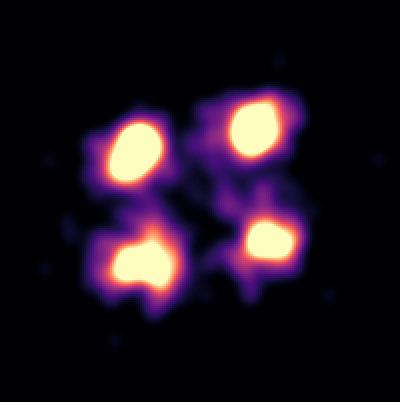
\includegraphics[width=\plotwidth]{figures/data/exp_counting/4bs_origami_1.png}
    \&
    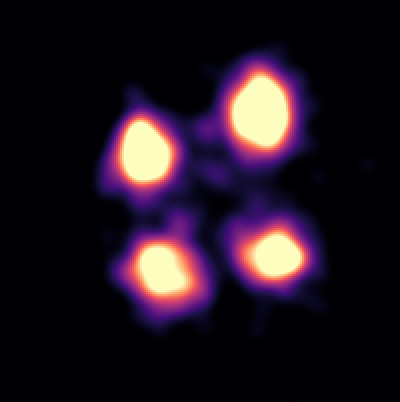
\includegraphics[width=\plotwidth]{figures/data/exp_counting/4bs_origami_2.png}
    \&
    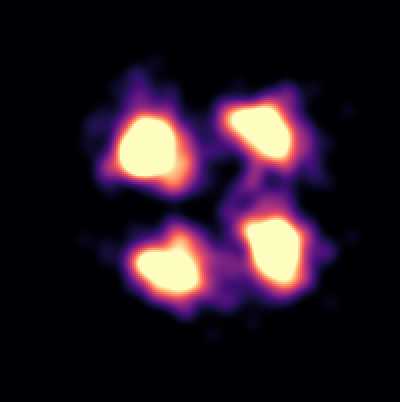
\includegraphics[width=\plotwidth]{figures/data/exp_counting/4bs_origami_3.png}
    \&
    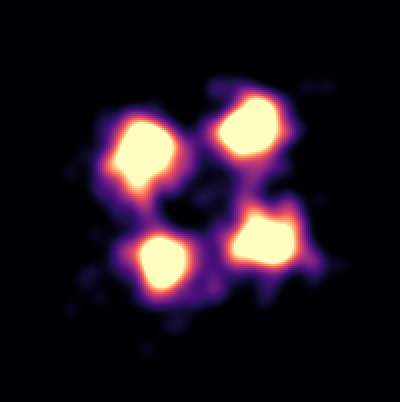
\includegraphics[width=\plotwidth]{figures/data/exp_counting/4bs_origami_4.png}
    \\
  };

  % scale bar
  \node[
    rectangle,
    minimum width=0.25\plotwidth, % images are 400px, 1/4 is 100px and that is 20nm
    fill=white,
    anchor=south east,
    inner sep=0pt,
    outer sep=2mm] (scalebar) at (samples-1-4.south east) {};
  \node[anchor=south,white] at (scalebar.center) {\tiny $20 \micrometer$};
\end{tikzpicture}
%
  \end{panel}
  \begin{panel}{(d)}{0.2\textwidth}
    \hspace{2mm}%
    \def\plotwidth{0.8\textwidth}%
    \def\plotheight{20mm}%
    \tikzsetnextfilename{exp_mean_probabilities_n1}%
\begin{tikzpicture}

  \pgfplotsset{every axis/.style={name=n1}}
  \def\posteriorcsv{figures/data/exp_counting/mean_probabilities.csv}
  \def\posteriorcol{n1_prob}
  \def\eps{0.001}%  skip bars for values below eps
\@ifundefined{noylabels}{}{
  \pgfplotsset{yticklabel=\empty}
  \pgfplotsset{ylabel=\empty}
}
\@ifundefined{noxlabel}{
  \pgfplotsset{xlabel=$n$}
}{
  \pgfplotsset{xlabel=\empty}
}
\begin{axis}[
  width=\plotwidth,
  height=\plotheight,
  scale only axis=true,
  enlarge x limits={abs=1.5},
  enlarge y limits=0,
  ymin=0,
  ymax=1,
  scaled ticks=false,
  ticklabel style={font=\tiny},
  xtick distance=1,
  axis background/.style={fill=white},
]

  \addplot+[
    ybar,
    bar width=1,
    mark=none,
    fill=posteriorcolor,
    fill opacity=0.6,
    draw=posteriorcolor,
    y filter/.expression={
      y < \eps ? nan : y
    },
  ] table [
    col sep=comma,
    y=\posteriorcol,
    x=n,
  ] {\posteriorcsv};

  \ifdefined\posteriorcolextra
    \addplot+[
      ybar,
      bar width=1,
      mark=none,
      fill=posteriorcolor!60!black,
      fill opacity=0.6,
      draw=posteriorcolor,
      y filter/.expression={
        y < \eps ? nan : y
      },
    ] table [
      col sep=comma,
      y=\posteriorcolextra,
      x=n,
    ] {\posteriorcsv};
  \fi

\end{axis}

  \node[anchor=south] at (n1.outer north) {origami with $\n=1$};

\end{tikzpicture}
%
  \end{panel}
  \begin{panel}{(e)}{0.2\textwidth}
    \hspace{2mm}%
    \def\plotwidth{0.8\textwidth}%
    \def\plotheight{20mm}%
    \tikzsetnextfilename{exp_mean_probabilities_n4}%
\begin{tikzpicture}

  \pgfplotsset{every axis/.style={name=n4}}
  \def\posteriorcsv{figures/data/exp_counting/mean_probabilities.csv}
  \def\posteriorcol{n4_prob}
  \def\eps{0.001}%  skip bars for values below eps
\@ifundefined{noylabels}{}{
  \pgfplotsset{yticklabel=\empty}
  \pgfplotsset{ylabel=\empty}
}
\@ifundefined{noxlabel}{
  \pgfplotsset{xlabel=$n$}
}{
  \pgfplotsset{xlabel=\empty}
}
\begin{axis}[
  width=\plotwidth,
  height=\plotheight,
  scale only axis=true,
  enlarge x limits={abs=1.5},
  enlarge y limits=0,
  ymin=0,
  ymax=1,
  scaled ticks=false,
  ticklabel style={font=\tiny},
  xtick distance=1,
  axis background/.style={fill=white},
]

  \addplot+[
    ybar,
    bar width=1,
    mark=none,
    fill=posteriorcolor,
    fill opacity=0.6,
    draw=posteriorcolor,
    y filter/.expression={
      y < \eps ? nan : y
    },
  ] table [
    col sep=comma,
    y=\posteriorcol,
    x=n,
  ] {\posteriorcsv};

  \ifdefined\posteriorcolextra
    \addplot+[
      ybar,
      bar width=1,
      mark=none,
      fill=posteriorcolor!60!black,
      fill opacity=0.6,
      draw=posteriorcolor,
      y filter/.expression={
        y < \eps ? nan : y
      },
    ] table [
      col sep=comma,
      y=\posteriorcolextra,
      x=n,
    ] {\posteriorcsv};
  \fi

\end{axis}

  \node[anchor=south] at (n4.outer north) {origami with $\n=4$};

\end{tikzpicture}
%
  \end{panel}

  \caption{
    \panelref{a, b} Experimental traces with super-resolution confirmed counts of one (a) and four (b), and \ours fits
    %
    \panelref{c} Super-resolution visualization of origamis made with four binding sites.
    %
    \panelref{d, e} Average \ours posterior distributions of 112 traces with a known $n$ of one (d) and 
    110 traces with a known $n$ of four (e)
  }
  \label{fig:results:experimental}
\end{figure*}


%-------------
\subsection{Simulated Experiments}
%-------------
% Simulated traces based on experimentally relevant parameters
Running \ours as a forward model to simulate experiment, 
we generated traces for counts $\n=1$ to 30 (\figref{fig:results:sim_counting}a,b).
	%
	We determined experimentally relevant camera parameters from a calibration of the
	sCMOS camera (\parametersc: $\camgain=2.17$, $\camoffset=4791$, $\camvar=774$). 
	%
	We determined kinetic (\parameterst: $\pon=0.036$, $\poff=0.028$), and emission parameters 
	(\parameterse: $\re=2.79$, $\rb=6.77$) from an initial experiment, 
	and these values closely matched those reported in the literature \cite{stein_2021}.
	%
	We simulated traces for 4000 frames, corresponding to an imaging time of 14 minutes.

% priors were placed on camera parameters, but all others were uniform
For inference, we placed tight empirically determined, Gaussian priors on 
the camera parameters.
	%
	We also placed flat uniform priors on the kinetic parameters, allowing the model 
	to fit blinking rates without external bias,
	%
	and loose priors on the emission parameters (\rb, \re) to prevent 
	over-estimation of count (see \secref{discussion}). 
	% how we got these priors
	We experimentally determined the prior on \rb by averaging the 
	intensity of the pixels immediately outside the region of interest.
	%
	We estimated the prior on \re  by first fitting a count of $\n=1$ to the trace.
	%
	The distribution of all observed $z$-states is unimodal.
	% 
	Therefore, whichever \z{}-state is the most common, the second most common state 
	will be $\z{} \pm 1$. 
	%
	We observed that fitting $n=1$ captures this specific transition, and provides a good
	estimate of photon emission rate of a single emitter \re.
	%
	
% blinx can count!
\ours accurately fit simulated traces with counts up to $\n=30$ (\figref{fig:results:sim_counting}c).
	%
	For $\n=10$ and below, \ours estimated the true count with a substantially 
	higher likelihood than all other possibilities. 
	%
	Above $\n=10$ the posterior broadened as other possibilities become more likely. 
	%
	The most likely estimate was the true count in 177/300 (59\%) of traces and 
	was within 1 of the true count in 267/300 (89\%) of all traces.
	%
	Importantly, in many cases \ours is able to fit the true count despite the fact that 
	not every state is occupied \ie the model is not just counting the 
	number of peaks in the intensity histogram (\figref{fig:results:sim_counting}a,b).
	% blinx outperforms lbFCS, counting up to 30 
	This is a tripling in performance compared to \lbfcs, which counted 
	accurately up to $\n=6$ and was within 1 of the true count for 64/300 (21\%) of traces 
	but failed to estimate higher counts.
	%
	Upon further analysis, the main limitation of \lbfcs is the estimation of the 
	intensity of a single emitter, corresponding to \re in \ours. 
	%
	\lbfcs relies on a histogram based method to determine this value, while 
	\ours is able to jointly optimize this parameter with the others.
	%
	Providing this value to \lbfcs led to a substantial recovery of performance.
	% 
	With \re provided, \lbfcs identified 200/300 (67\%) of traces within 1 of the true count. 
	%

Both \ours and \lbfcs achieve this counting accuracy without prior knowledge of the kinetic parameters.
	%
	In contrast, \qpaint is heavily dependant on a kinetic calibration and 
	therefore not comparable in this context.
	%
	A direct comparison to \qpaint is shown in \secref{results:qpaint}

% Longer traces lead to better fits
A longer trace provides more
information to the model and increases the counting accuracy.
	%
	We simulated and fit traces of lengths ranging from 100 to 10,000 frames, with the same parameters 
	as the previous section (\figref{fig:results:sim_counting}d).
	%
	As expected, accuracy increased and variance of the posterior distribution decreased, 
	as trace length increased.
	% Also notice a underestimation of count with low trace length
	Interestingly for short trace lengths, \ours consistently underestimated the true count. 
	% This is most likely due to the system only occupying a subset of all possible zs in this short time
	This is likely because only a subset of possible states were observed in this short time. % maybe more explanation?

% there is a lower bound to SNR, below a specific SNR, model maximally overcounts
We determined the robustness of our model and the minimum signal-to-noise ratio 
(SNR) needed to achieve an accurate count.
	%
	We artificially increased the variance of the readout noise \camvar, 
	to simulate traces with SNRs ranging from 9 to 1 (where 9 
	corresponds to the parameters previously used).
	%
	Because noise in our model is a function of intensity, quantifying the SNR of a trace 
	is not trivial. 
	%
	For simplicity, here we define SNR as the difference in intensity between 
	the first two states (\z{0} and \z{1}) divided by the standard deviation of the difference. 
	%
	In effect this is the higher bound of SNR for a given trace. 
	%
	\ours shows accurate counting for SNRs $\geq 4$ (\figref{fig:results:sim_counting}e). 
	%
	Interestingly, for  SNR $\leq 4$, \ours estimates the count as 25, 
	the highest \n tested, no matter the true count. 
	%
	This is due to the model adding states to compensate for the wide distribution of intensities  
	(see \secref{discussion}).

%-------------
\subsection{Effect of kinetic parameters}
%-------------
The performance of our model depends on the true kinetic parameters of the system (\pon and \poff).
%
	To find a regime that maximizes our models counting ability, we simulated and fit traces 
	from $\n=1$ to 20, with a range of kinetic parameters, 
	while holding all other parameters constant.
	%
	We ensured that this range covered experimentally relevant kinetics from the literature including:
	qPAINT: (\pon, \poff) = (0.006, 0.2) \cite{jungmann_2016} and \lbfcs (0.02, 0.02) \cite{stein_2021}. 
	%
	We summarized the resulting posteriors by calculating the expected squared error over all true counts: 
	$\sum w(\truen - \n)^2$, where $w$ is the probability of the estimated count \n 
	(\figref{fig:results:campare_kinetics}a).

The result can be divided into two clear regimes: $\pon < \poff$ and $\pon \geq \poff$.
	%
	In the first regime, where $\pon < \poff$ we see significant limitations to our models counting ability.
	%
	Furthermore, when \pon is substantially lower than \poff, our model loses almost 
	all ability to count and estimates $\truen=1$ or 2, regardless of the true $\truen$.
	%
	In contrast, in the second regime, where $\pon \geq \poff$ we observe 
	accurate counting up to $n=20$.
	%
	A clear difference between these two regimes can be seen in the distribution 
	of their hidden states \z{} (\figref{fig:results:campare_kinetics}a, insets).
	%
	When $\pon < \poff$, the distribution is shifted towards 0, and a majority 
	of the frames occupy the lowest two \z{}-states (\figref{fig:results:campare_kinetics}c). 
	In this regime, the true count becomes indistinguishable for all methods, without prior information. 
	%
	When $\pon \geq \poff$, this distribution is centered, or even shifted towards $n$ 
	and a larger fraction of the states are visited (\figref{fig:results:campare_kinetics}d). 
	%
	This provides ample information for the model to infer the correct $n$.
	
% Experimental
% Do we need to explain how DNA-PAINT works
In DNA-PAINT, the blinking rate is determined by the kinetics of single-stranded DNA binding,
which in turn depends on experimental conditions such as temperature and concentration, 
and the specific DNA sequence~\citep{jungmann_single-molecule_2010}.
	%
	As a result, the kinetic parameters \pon and \poff of our model can be 
	tuned by adjusting the temperature and imager concentration (\figref{fig:results:campare_kinetics}b).
	%
	We imaged DNA origami with a known count of $\n=1$ at 25\textdegree C and an 
	imager concentration of 10 nM and measured $\pon=0.028$ and $\poff=0.072$ 
	(\figref{fig:results:campare_kinetics}b),
	%
	which places these conditions firmly in the poor counting 
	accuracy regime of $\pon < \poff$ (\figref{fig:results:campare_kinetics}a). % fix
	%
	To move to a more favorable kinetic regime for experiments, 
	we increased the imager concentration and decreased the temperature.
	%
	Increasing imager concentration to 30 nM raised \pon to 0.071 and 
	decreasing temperature to 13\textdegree C decreased \poff to 0.037 
	(\figref{fig:results:campare_kinetics}b).
	%
	As expected, he effects of temperature and concentration were largely independent 
	of one another \cite{jungmann_single-molecule_2010}.
	%
	We also observed a substantial decrease in SNR with decreasing temperature 
	and with increasing concentration. 
	%
	This was an expected side effect of increasing concentration, because increasing 
	imager concentration increases \rb.
	%
	But the effect of temperature on SNR was surprising. 
	We hypothesize that this is due to the stabilization of partial 
	binding between imager and docker strands at low temperatures.
	%
	Accounting for both the increase in counting accuracy and the decrease 
	in SNR, we identified imaging conditions of 20 nM and 13\textdegree C as 
	optimal on our microscope.

%-------------
\subsection{qPAINT Kinetic Regime} \label{results:qpaint}
%-------------
% qPAINT operates in a different kinetic regime that lbFCS
qPAINT relies on the accurate measurement of the average dark time between blinking events~\citep{jungmann_2016} 
	%
	and is therefore optimized for an entirely different kinetic regime, where blinking 
	events are short and infrequent (\figref{fig:results:qpaint_counting}a,b).
	% 
	This regime presents a challenge to \ours (\figref{fig:results:campare_kinetics}a top inset). 
	%
	If the only states ever observed are $\z{}=0$ or 1, there is insufficient 
	information to estimate count without prior knowledge.
	% 
	qPAINT faces the same limitation and relies on a calibration 
	of the blinking kinetics of a single binding site.
	% 
	\ours, being a Bayesian model can incorporate a similar calibration 
	as priors of the kinetic parameters.
	%
	With this addition, and the tightening of the priors on \re and \rb, the counting 
	accuracy of \ours is restored (\figref{fig:results:qpaint_counting}c). 
	%
	\ours estimated the true count as the most likely in 133/300 (44\%) of traces and 
	estimated within 1 of the true count in 269/300 (90\%) of all traces,
	comparable to the favorable kinetic regime (\figref{fig:results:sim_counting}c).
	%
	However, obtaining these priors requires additional experimental steps, and is often not trivial. 
	%
	Thus, a tradeoff exists.
	%
	Without any calibration, \ours is able to accurately count in a subset of kinetic 
	conditions where $\pon > \poff$.
	%
	But with an experimental calibration, the counting ability of \ours is expanded 
	to a wider range of kinetic conditions. 

% qPAINT undercounts but blinx does not
Due to the stochastic nature of blinking, multiple emitters can 
be active at any given time-point, which becomes increasingly likely at higher counts.
	%
	This is not compatible with the qPAINT requirement of well separated, 
	single emitter blinking events.
	%
	As a result at higher \n the measured average dark time is longer than the true average dark time
	and  results in qPAINT underestimating molecular count at higher \n
	(especially noticeable above $\n=20$, see \figref{fig:results:qpaint_counting}c). 
	%
	In \ours, the activity of multiple emitters at a single timepoint is explicitly modeled in both the 
	intensity and transition models previously derived (\eqref{eq:methods:p_c_given_z} and \eqref{eq:method:transition}). 
	%
	As a result, \ours avoids underestimating, and provides an accurate measurement 
	of the molecular count up to $\n=30$.
	
%-------------
\subsection{Experimental Counting}
%-------------
% briefly describe experimental setup
To experimentally validate the counting performance of \ours, we used DNA-Origami, 
which provides nano-scale control over the number and location of emitters~\citep{rothemund_folding_2006}.
	% Why DNA origami
	DNA-Origamis were designed containing 1 and 4 DNA-PAINT docker strands, 
	spaced in a grid 20 \nanometer apart. 
	%
	This distance was chosen so that the true number of docker strands 
	could be visually confirmed through super-resolution post-processing.
	%
	Incorporation efficiency is roughly 80 percent for each docker site \cite{strauss_2018}, 
	so only a fraction of the origamis were expected to contain all 4 dockers. 
	% 
	Origamis were first imaged at 13\textdegree C with low laser power (1.5\%) and 20 nM imager concentration to 
	collect traces (4,000 frames at 200 ms exposure time) for counting with \ours (\figref{fig:results:experimental}a,b).
	%
	The system was then allowed to warm to 25\textdegree C a buffer exchange was performed, and new imager 
	was added at 10 nM.
	%
	The origamis were imaged again at high laser power (40\%),
	and post-processed with Picasso \citep{schnitzbauer_2017} to obtain super-resolution ground truth (\figref{fig:results:experimental}c).
	%
	Only origamis that had a visual count matching the designed count (1 or 4) were selected for analysis with \ours.

Of the 131 traces with a known count of 1, \ours correctly counted 112 (85\%)
and the average of the posterior distributions is shown in \figref{fig:results:experimental}d.
	%
	Possible counts up to $\n=8$ were modelled, but the likelihoods for counts above $n=3$ were negligible for all traces.
	%
	For the traces with a known count of 4, 71/110 (65\%) were correctly identified as 4, 
	and 103/110 were identified as between 3 and 5. 
	%
	The average posterior distribution is shown in \figref{fig:results:experimental}e.
	Importantly, traces were not preprocessed or filtered before undergoing \ours counting analysis.
